\documentclass[12pt]{article}

\usepackage{tikz} % картинки в tikz
\usepackage{microtype} % свешивание пунктуации
\usepackage{array} % для столбцов фиксированной ширины
\usepackage{comment} % для комментирования целых окружений
\usepackage{indentfirst} % отступ в первом параграфе

\usepackage{sectsty} % для центрирования названий частей
\allsectionsfont{\centering}

\usepackage{amsmath, amssymb, amsthm, amsfonts} % куча стандартных математических плюшек

\usepackage[top=2cm, left=1cm, right=1cm, bottom=2cm]{geometry} % размер текста на странице
\usepackage{lastpage} % чтобы узнать номер последней страницы
 
\usepackage{enumitem} % дополнительные плюшки для списков
%  например \begin{enumerate}[resume] позволяет продолжить нумерацию в новом списке

\usepackage{caption} % подписи к рисункам
\usepackage{hyperref} % гиперссылки
\usepackage{multicol} % текст в несколько столбцов


\usepackage{fancyhdr} % весёлые колонтитулы
\pagestyle{fancy}
\lhead{Введение в машинное обучение, ВШЭ}
\chead{}
\rhead{2022-04-01}
\lfoot{Вариант $\pi$}
\rfoot{Паниковать запрещается!}
%\rfoot{Тест}
\renewcommand{\headrulewidth}{0.4pt}
\renewcommand{\footrulewidth}{0.4pt}

\usepackage{ifthen} % для написания условий

\usepackage{todonotes} % для вставки в документ заметок о том, что осталось сделать
% \todo{Здесь надо коэффициенты исправить}
% \missingfigure{Здесь будет Последний день Помпеи}
% \listoftodos --- печатает все поставленные \todo'шки


% более красивые таблицы
\usepackage{booktabs}
% заповеди из докупентации:
% 1. Не используйте вертикальные линни
% 2. Не используйте двойные линии
% 3. Единицы измерения - в шапку таблицы
% 4. Не сокращайте .1 вместо 0.1
% 5. Повторяющееся значение повторяйте, а не говорите "то же"


\usepackage{fontspec}
\usepackage{polyglossia}

\setmainlanguage{russian}
\setotherlanguages{english}

% download "Linux Libertine" fonts:
% http://www.linuxlibertine.org/index.php?id=91&L=1
\setmainfont{Linux Libertine O} % or Helvetica, Arial, Cambria
% why do we need \newfontfamily:
% http://tex.stackexchange.com/questions/91507/
\newfontfamily{\cyrillicfonttt}{Linux Libertine O}

% Математические шрифты 
% Математические шрифты 
\usepackage{unicode-math}     
\setmathfont[math-style=upright]{euler.otf} 

\setmathfont[range={\mathbb, \mathop, \heartsuit, \angle, \smile, \varheartsuit}]{Asana-Math.otf}

\AddEnumerateCounter{\asbuk}{\russian@alph}{щ} % для списков с русскими буквами
\setlist[enumerate, 2]{label=\asbuk*),ref=\asbuk*}


% мои цвета https://www.artlebedev.ru/colors/
\definecolor{titleblue}{rgb}{0.2,0.4,0.6} 
\definecolor{blue}{rgb}{0.2,0.4,0.6} 
\definecolor{red}{rgb}{1,0,0.2} 
\definecolor{green}{rgb}{0,0.6,0} 
\definecolor{purp}{rgb}{0.4,0,0.8} 

% цвета из geogebra 
\definecolor{litebrown}{rgb}{0.6,0.2,0}
\definecolor{darkbrown}{rgb}{0.75,0.75,0.75}

% Гиперссылки
\usepackage{xcolor}   % разные цвета

\usepackage{hyperref}
\hypersetup{
  unicode=true,           % позволяет использовать юникодные символы
  colorlinks=true,        % true - цветные ссылки
  urlcolor=blue,          % цвет ссылки на url
  linkcolor=black,          % внутренние ссылки
  citecolor=green,        % на библиографию
  breaklinks              % если ссылка не умещается в одну строку, разбивать её на две части?
}

% эпиграфы
\usepackage{epigraph}
\setlength\epigraphwidth{.35\textwidth}
\setlength\epigraphrule{0pt}

% Математические операторы первой необходимости:
\DeclareMathOperator{\sgn}{sign}
\DeclareMathOperator*{\argmin}{arg\,min}
\DeclareMathOperator*{\argmax}{arg\,max}
\DeclareMathOperator{\Cov}{Cov}
\DeclareMathOperator{\Var}{Var}
\DeclareMathOperator{\Corr}{Corr}
\DeclareMathOperator{\E}{\mathop{E}}
\DeclareMathOperator{\Med}{Med}
\DeclareMathOperator{\Mod}{Mod}
\DeclareMathOperator*{\plim}{plim}

\DeclareMathOperator{\logloss}{logloss}
\DeclareMathOperator{\softmax}{softmax}

\DeclareMathOperator{\tr}{tr}

% команды пореже
\newcommand{\const}{\mathrm{const}}  % const прямым начертанием
\newcommand{\iid}{\sim i.\,i.\,d.}  % ну вы поняли...
\newcommand{\fr}[2]{\ensuremath{^{#1}/_{#2}}}   % особая дробь
\newcommand{\ind}[1]{\mathbbm{1}_{\{#1\}}} % Индикатор события
\newcommand{\dx}[1]{\,\mathrm{d}#1} % для интеграла: маленький отступ и прямая d

% одеваем шапки на частые штуки
\def \hb{\hat{\beta}}
\def \hs{\hat{s}}
\def \hy{\hat{y}}
\def \hY{\hat{Y}}
\def \he{\hat{\varepsilon}}
\def \hVar{\widehat{\Var}}
\def \hCorr{\widehat{\Corr}}
\def \hCov{\widehat{\Cov}}

% Греческие буквы
\def \a{\alpha}
\def \b{\beta}
\def \t{\tau}
\def \dt{\delta}
\def \e{\varepsilon}
\def \ga{\gamma}
\def \kp{\varkappa}
\def \la{\lambda}
\def \sg{\sigma}
\def \tt{\theta}
\def \Dt{\Delta}
\def \La{\Lambda}
\def \Sg{\Sigma}
\def \Tt{\Theta}
\def \Om{\Omega}
\def \om{\omega}

% Готика
\def \mA{\mathcal{A}}
\def \mB{\mathcal{B}}
\def \mC{\mathcal{C}}
\def \mE{\mathcal{E}}
\def \mF{\mathcal{F}}
\def \mH{\mathcal{H}}
\def \mL{\mathcal{L}}
\def \mN{\mathcal{N}}
\def \mU{\mathcal{U}}
\def \mV{\mathcal{V}}
\def \mW{\mathcal{W}}

% Жирные буквы
\def \mbb{\mathbb}
\def \RR{\mbb R}
\def \NN{\mbb N}
\def \ZZ{\mbb Z}
\def \PP{\mbb{P}}
\def \QQ{\mbb Q}

\def \putyourname{\fbox{
    \begin{minipage}{42em}
      Фамилия, имя, номер группы:\vspace*{3ex}\par
      \noindent\dotfill\vspace{2mm}
    \end{minipage}
  }
}

\def \checktable{

  \vspace{5pt}
  Табличка для проверяющих работу:

\vspace{5pt}

  \begin{tabular}{|m{2cm}|m{1cm}|m{1cm}|m{1cm}|m{1cm}|m{1cm}|m{2cm}|}
\toprule
    Тест & 1 &  2 & 3 & 4 & 5 & Итого \\
\midrule
    &  &  & & & & \\
    &  &  & & & & \\
 \bottomrule
\end{tabular}
}


\def \testtable{

\vspace{5pt}
  Внесите сюда ответы на тест:

\vspace{5pt}

\begin{tabular}{|m{2cm}|m{0.6cm}|m{0.6cm}|m{0.6cm}|m{0.6cm}|m{0.6cm}|m{0.6cm}|m{0.6cm}|m{0.6cm}|m{0.6cm}|m{0.6cm}|}
\toprule
    Вопрос & 1 &  2 & 3 & 4 & 5 & 6 & 7 & 8 & 9 & 10 \\
\midrule
    Ответ &  &  & & & & & & & & \\
 \bottomrule
\end{tabular}
}


% [1][3] 1 = one argument, 3 = value if missing
% эта магия создаёт окружение answerlist
% именно в окружении answerlist записаны варианты ответов в подключаемых exerciseXX
% просто \begin{answerlist} сделает ответы в три столбца
% если ответы длинные, то надо в них руками сделать
% \begin{answerlist}[1] чтобы они шли в один столбец
\newenvironment{answerlist}[1][3]{
\begin{multicols}{#1}

\begin{enumerate}[label=\fbox{\emph{\Alph*}},ref=\emph{\alph*}]
}
{
\item Нет верного ответа.
\end{enumerate}
\end{multicols}
}

% BB: unicol version. don't know why \ifthenelse fails in second part of new-env
\newenvironment{answerlistu}{
\begin{enumerate}[label=\fbox{\emph{\Alph*}},ref=\emph{\alph*}]
}
{
\item Нет верного ответа.
\end{enumerate}
}


\excludecomment{solution} % without solutions

\theoremstyle{definition}
\newtheorem{question}{Вопрос}

\usepackage{tikzlings}
\usepackage{tikzducks}

\usepackage{alltt}

\begin{document}

\putyourname

\testtable

\checktable

\mbox{ }

\epigraph{Совы не то, чем они кажутся {\tikz[scale=0.5]\owl;}}{\textit{Великан из Твин Пикс (1990)}}

\textbf{Это нулевой вариант мидтёрма. Он нужен для того, чтобы его формат не стал для вас сюрпризом.} Работа состоит из трёх частей: тестовая, задачи и ответы на открытые вопросы. Списывание карается обнулением работы. Удачи!


%  Распределение тем для тестов (30 баллов)

%  1.  Что-то про постановку задачи (какие бывают)
%  2.  Оценка качества модели (выборки кросс-валидации и тп)
%  3.  Измерение качества модели
%  4.  Градиентный спуск
%  5.  Предобработка данных 
%  6.  Что-то про линейную регрессию 
%  7.  Что-то про регуляризацию 
%  8.  Что-то про классификацию
%  9.  Что-то про логистическую регрессию
%  10. Что-то про метрики классификации


% Распределение тем для открытых вопросов  (50 баллов)

% 1. Дано описание задачи. Надо выписать к какому типу она относится, что таргет, что объекты, что признаки. 
% 2. Какие-нибудь формулы и в них надо найти все ошибки
% 3. Записать какую-нибудь модель и объяснить как она работает
% 4. Объяснить мем (надо намайнить простых мемов)
% 5. Что-то про то как чел учил модель и облажался. Где облажался и как фиксить? 


% Распределение тем для ручных задач  (20 баллов)

% 1. Расчёт каких-нибудь метрик (классификация/регрессия) и тп 
% 2. Задача, которую надо решить чтобы добить оценку до 10 (для лучших) 


\section*{Часть первая: тестовая} 

Дайте ответ на $10$ тестовых вопросов. Каждый вопрос стоит $3$ балла. Никакие дополнительные пояснений в этой части работы от вас не требуются.


\begin{question}
У Ратибора есть онлайн-кинотеатр с огромным количеством фильмов. Ратибор знает жанры для каждого из них. В понедельник база фильмов пополнится новыми релизами студии Disney. К сожалению, новые фильмы придут без указанных жанров. Ратибор хочет предсказать их с помощью машинного обучения. Какую задачу ему предстоит решить? 
\begin{answerlist}
  \item  Кластеризаия
  \item  Классификация {\tikz[scale=0.25]\owl;}
  \item  Регрессия
  \item  Ранжирование
  \item  Рекомендации
\end{answerlist}
\end{question}

\begin{solution}
\begin{answerlist}
  \item Bad answer :(
  \item Good answer :)
  \item Bad answer :(
  \item Bad answer :(
  \item Bad answer :(
\end{answerlist}
\end{solution}


\begin{question}
Качество чего оценивается с помощью кросс-валидации или отложенной выборки?
\begin{answerlist}
  \item Метода обучения параметров для конкретной модели
  \item Конкретной обучающей выборки
  \item Конкретного набора признаков
  \item Регуляризации
  \item Модели с конкретным набором параметров {\tikz[scale=0.25]\owl;}
\end{answerlist}
\end{question}

\begin{solution}
\begin{answerlist}
  \item Bad answer :(
  \item Bad answer :(
  \item Bad answer :(
  \item Bad answer :(
  \item Good answer :)
\end{answerlist}
\end{solution}

\newpage 

\begin{question}
Допустим, мы обучаем линейную модель на $MSE$ с $L_2$-регуляризатором. Как будет разумно измерять её ошибку на тестовой выборке?
\begin{answerlist}
  \item Из~$MSE$~надо~вычесть значение $L_2$-регуляризатора
  \item По~$MSE$~с~$L_2$-регуляризатором
  \item По~значению~$L_2$ регуляризатора
  \item По $MSE$ {\tikz[scale=0.25]\owl;}
  \item Подойдёт любой из вышеперечисленных способов
\end{answerlist}
\end{question}

\begin{solution}
\begin{answerlist}
  \item Bad answer :(
  \item Bad answer :(
  \item Bad answer :(
  \item Good answer :)
  \item Bad answer :(
\end{answerlist}
\end{solution}


\begin{question}
Выберите верные утверждения про стохастический градиентный спуск
\begin{answerlist}
  \item В SGD, скорее всего, потребуется больше итераций для сходимости, чем в обычном градиентном спуске {\tikz[scale=0.25]\owl;}
  \item SGD НЕ используется в современном машинном обучении
  \item В SGD одна итерация требует больше вычислений, чем в обычном градиентном спуске
  \item В SGD, скорее всего, потребуется меньше итераций для сходимости, чем в обычном градиентном спуске
  \item В SGD одна итерация требует меньше вычислений, чем в обычном градиентном спуске {\tikz[scale=0.25]\owl;}
\end{answerlist}
\end{question}

\begin{solution}
\begin{answerlist}
  \item Good answer :)
  \item Bad answer :(
  \item Bad answer :(
  \item Bad answer :(
  \item Good answer :)
\end{answerlist}
\end{solution}


\begin{question}
Какие из сопособов приведённых ниже можно использовать для работы с пропусками в действительных переменных при обучении линейных моделей? 
\begin{answerlist}
   \item Если пропусков очень много, выкинуть переменную {\tikz[scale=0.25]\owl;}
   \item Заполнить пропуски аномальным значением
   \item Выделить пропуски в отдельную категорию и сделать OHE-преобразование
  \item Заполнить нулями {\tikz[scale=0.25]\owl;}
  \item Заполнить пропуски медианами, посчитанными по каждой колонке {\tikz[scale=0.25]\owl;}
\end{answerlist}
\end{question}

\begin{solution}
\begin{answerlist}
  \item Good answer :)
  \item Bad answer :(
  \item Bad answer :(
  \item Good answer :)
  \item Good answer :)
\end{answerlist}
\end{solution}


\begin{question}
Драгомир пытается предсказать продажи видео-игр. Он предсказыват продажи по возрасту игры, $x$. Целевая переменная $y$ --- количество продаж. Драгомир оценил линейную регрессию: 

$$ 
\ln y = 5 - 6 \cdot  \ln x.
$$

Предположим, что мы отгружаем на рынок новую партию игры, выпущенной в прошлом году. Спрогнозируйте, сколько экземпляров этой игры будет продано? 

\begin{answerlist}
  \item \( 4 \)
  \item \( 20 \)
  \item \( 148 \) {\tikz[scale=0.25]\owl;}
  \item \( 5 \)
  \item \( 0 \) 
\end{answerlist}
\end{question}

\begin{solution}
\begin{answerlist}
  \item Bad answer :(
  \item Bad answer :(
  \item Good answer :)
  \item Bad answer :(
  \item Bad answer :(
\end{answerlist}
\end{solution}


\begin{question}
Выберите все верные утверждения про регуляризацию линейных моделей.
\begin{answerlist}
  \item Регуляризация штрафует модель за слишком \textbf{большие} по модулю значения коэффициентов {\tikz[scale=0.25]\owl;}
  \item $L_2$-регуляризация зануляет коэффициенты
  \item Регуляризация штрафует модель за слишком \textbf{маленькие} по модулю значения кожффициентов
  \item $L_1$-регуляризация зануляет коэффициенты {\tikz[scale=0.25]\owl;}
  \item Регуляризатор обычно приплюсовывают к функции потерь {\tikz[scale=0.25]\owl;}
\end{answerlist}
\end{question}

\begin{solution}
\begin{answerlist}
  \item Bad answer :(
  \item Good answer :)
  \item Bad answer :(
  \item Good answer :)
  \item Bad answer :(
\end{answerlist}
\end{solution}

\newpage 

\begin{question}
Велимудр обучает метод ближайших соседей для классификации молекул на токсичные и обычные. Выберите все верные утверждения про KNN:
\begin{answerlist}
  \item  Велимудр может подобрать оптимальное число соседей с помощью кросс-валидации {\tikz[scale=0.25]\owl;}
  \item  Для обучения KNN важно отнормировать данные {\tikz[scale=0.25]\owl;}
  \item  KNN на этапе обучения подбирает оптимальное число соседей с помощью градиентного спуска
  \item  KNN на этапе обучения запоминает выборку {\tikz[scale=0.25]\owl;}
  \item  Если взять число соседей очень большим, модель точно не переобучится
\end{answerlist}
\end{question}

\begin{solution}
\begin{answerlist}
  \item Good answer :)
  \item Good answer :)
  \item Bad answer :(
  \item Good answer :)
  \item Bad answer :(
\end{answerlist}
\end{solution}


\begin{question}
Рагнеда классифицирует фотографии. Она хочет обучить логистическую регрессию, которая будет отличать гусей от уток. Пусть $\hat p_i$ --- это предсказание вероятности того, что на фото гусь, $y_i = 1,$ если на фото гусь.  Какую функцию потерь надо минимизировать Рагнеде для обучения модели? 
\begin{answerlist}
  \item  $p_i \cdot \ln (1 - y_i) + (1 - p_i) \cdot \ln y_i$ 
  \item  $y_i \cdot \ln (1 - p_i) + (1 - y_i) \cdot \ln  p_i$
  \item  $y_i \cdot \ln p_i + (1 - y_i) \cdot \ln (1 - p_i) {\tikz[scale=0.25]\owl;}$ 
  \item  $p_i \cdot \ln y_i + (1 - p_i) \cdot \ln (1 - y_i)$
  \item  $(y_i - \hat p_i)^2$
\end{answerlist}
\end{question}

\begin{solution}
\begin{answerlist}
  \item Good answer :)
  \item Bad answer :(
  \item Bad answer :(
  \item Bad answer :(
  \item Bad answer :(
\end{answerlist}
\end{solution}


\begin{question}
Выберите все метрики классификации, которые не зависят от выбора порога 
\begin{answerlist}
  \item Доля правильных ответов (accuracy)
  \item Точность (precision)
  \item Площадь под ROC-кривой (ROC-AUC)~{\tikz[scale=0.25]\owl;}
  \item f-мера
  \item Площадь под PR-кривой (PR-AUC)~{\tikz[scale=0.25]\owl;}
\end{answerlist}
\end{question}

\begin{solution}
\begin{answerlist}
  \item Bad answer :(
  \item Bad answer :(
  \item Good answer :)
  \item Bad answer :(
  \item Good answer :)
\end{answerlist}
\end{solution}


\newpage 

 
\section*{Часть вторая: открытые вопросы}

Эта часть состоит из открытых вопросов. На них необходимо дать краткие, но ёмкие ответы. За каждый ответ вы можете получить 10 баллов.

\begin{question}
Предложите для каждой из перечисленных ниже задач, как сформулировать их в терминах машинного обучения: укажите, что будет являться объектом и целевой переменной, а также напишите тип задачи.

\begin{enumerate}
    \item Мы делаем сервис доставки еды. Мы хотим показывать пользователю, который собирает заказ, через сколько этот заказ будет доставлен. 

    \item Служба поддержки в одном сервисе такси не справляется с нагрузкой. Однако некоторые запросы связаны с тем, что клиент забыл в машине документы или вещи, поэтому надо быстрее помочь ему связаться с водителем. Мы хотим с помощью машинного обучения определять по запросу, стоит ли рассматривать его в первую очередь.
\end{enumerate}
\end{question}


\vspace{4cm} 


\begin{question}
Машинлёрнерша Рагнеда не доверяет пакетным реализациям алгоритмов машинного обучения. Поэтому она написала свой собственный градиентный спуск. Для того, чтобы делать шаг градиентного спуска, она использовала следующие формулы. 

\[
w_t = w_{t - 1} + (\nabla Q(w_{t}))^2
% w_t = w_{t-1} - \gamma_t \cdot \nabla Q(w_{t-1})
\]


Какие ошибки вы тут видите? Для каждой объясните, к каким последствиям и почему она приведёт, а также как это исправить.
\end{question}


\vspace{4cm} 
\newpage 

\begin{question}
Объясните мем
\begin{center}
  
\includegraphics[scale=0.2]{mem1.jpg}
\end{center}
\end{question}

\vspace{4cm} 


\begin{question}
Результатом обучения логистической регрессии является вектор весов $w$. Если нам дан объект $x$, как посчитать вероятность того, что он относится к положительному классу? Объясните все компоненты в формуле, которую запишите.
\end{question}


\newpage 

\begin{question}
Доброгнева обучает линейную регрессию для предсказания цен на недвижимость. Она хочет, чтобы коэффициенты перед соотвествующими факторами отражали их важность для итогового прогноза. На левой картинке Доброгнева построила значения коэффициентов. На правой она визуализировала стандартное отклонение каждого фактора. Добилась ли Доброгнева нужной ей интерпретации коэффициентов? Что они в действительности отражают? Как это исправить? 

\begin{center}
  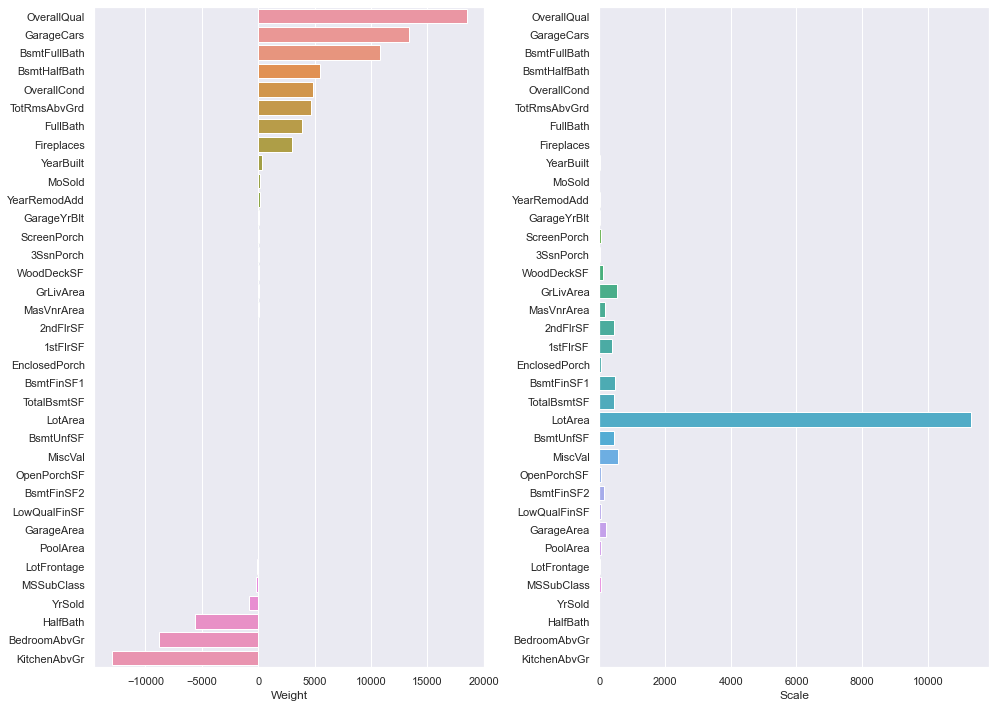
\includegraphics[scale=0.5]{scale.png}
\end{center}
\end{question}


\newpage 


\section*{Часть третья: задачки}

Решите все задания. Все ответы должны быть обоснованы. Решения должны быть прописаны для каждого пункта. Рисунки должны быть чёткими и понятными. Все линии должны быть подписаны. За решение каждой задачи вы можете получить 10 баллов.

\begin{question}
Винни-Пух и Пятачок классифицируют пчёл на правильных и неправильных. У них есть выборка $X$, состоящая из $7$ объектов, и классификатор $a(x),$ предсказывающий оценку принадлежности пчелы к правильным. Предсказания $a(x)$ и реальные метки пчёл представлены ниже: 

\begin{table}[h]
    \centering
    \begin{tabular}{>{\bfseries}cccccccc}
        \toprule
         b(x) & 0.2 & 0.6 & 0.3 & 0.7 & 0.5 & 0.9 & 0.6  \\ \midrule
         y & -1 & +1 & -1 & -1 & +1 & +1 & -1 \\
         \bottomrule
    \end{tabular}
\end{table}

\begin{enumerate}
    \item Пятачок считает, что порог $t=0.55$ самый лучший. Вычислите precision и recall для такого классификатора. 

    \item Винни-Пух согласен с Пяточком, но у него в голове опилки. При подсчёте тех же метрик он перепутал местами предсказания классификатора и реальные метки. Какие значения метрик он получит?
    
    \item Что будет происходить с precision и recall, если Винни-Пух и Пяточок увеличат порог? 
\end{enumerate}
\end{question}

\newpage 

\begin{question}
На плоскости расположены колонии рыжих и чёрных муравьёв. Рыжих колоний три и они имеют координаты $(-1, -1)$, $(1, 1)$ и $(3, 3)$. Чёрных колоний тоже три и они имеют координаты $(2, 2)$, $(4, 4)$ и $(6, 6)$.

\begin{enumerate}
  \item[а)] Поделите плоскость на «зоны влияния» рыжих и чёрных муравьёв, используя метод одного ближайшего соседа (надо явно указать как будет классифицирована каждая точка плоскости и провести разделяющую поверхность). 
  \item[б)] Поделите плоскость на «зоны влияния» рыжих и чёрных муравьёв, используя метод трёх ближайших соседей.
  \item[в)] С помощью кросс-валидации с выкидыванием отдельных наблюдений выберите оптимальное число соседей $k$ перебрав $k \in \{1, 3, 5\}$. Целевой функцией является количество верных предсказаний (accuracy).
\end{enumerate}
\end{question}


\end{document}
